\section{LLMs for Phone Automation}
\label{sec:models}

LLMs~\cite{radford2018gpt1,radford2019gpt2,brown2020gpt3,achiam2023gpt} have emerged as a transformative technology in phone automation, bridging natural language inputs with executable actions. By leveraging their advanced language understanding, reasoning, and generalization capabilities, LLMs enable agents to interpret complex user intents, dynamically interact with diverse mobile applications, and effectively manipulate GUIs.

In this section, we explore two primary approaches to leveraging LLMs for phone automation: \textbf{Training-Based Methods} and \textbf{Prompt Engineering}. Figure~\ref{fig:model_differences} illustrates the differences between these two approaches in the context of phone automation. \textbf{Training-Based Methods} involve adapting LLMs specifically for phone automation tasks through techniques like supervised fine-tuning~\cite{cheng2024seeclick, chen2024guicourse, lu2024guiodyssey, pawlowski2024tinyclick} and reinforcement learning~\cite{song2024trial, bai2024digirl, wang2024distrl}. These methods aim to enhance the models' capabilities by training them on GUI-specific data, enabling them to understand and interact with GUIs more effectively. \textbf{Prompt Engineering}, on the other hand, focuses on designing input prompts to guide pre-trained LLMs to perform desired tasks without additional training~\cite{wei2022chain, yao2024tree, chen2022program}. By carefully crafting prompts that include relevant information such as task descriptions, interface states, and action histories, users can influence the model's behavior to achieve specific automation goals~\cite{wen2023droidbot, zhang2023appagent, song2023navigating}.

\begin{figure*}[ht]
    \centering
    \includegraphics[width=0.95\linewidth]{figures/pe_process.drawio.png}
    \caption{
        Schematic of prompt engineering for phone automation. 
        The \textbf{\textcolor[RGB]{184,84,80}{necessary prompt}} is mandatory, initiating the task, e.g., searching for a Korean restaurant. 
        The \textbf{\textcolor[RGB]{130,179,102}{optional prompt}} are supplementary, enhancing tasks without being mandatory. 
        The \textbf{\textcolor[RGB]{14,128,139}{flexible prompt}} must include one or more elements from the UI Info, like a screenshot or OCR info, to adapt to task needs.
    }
    \label{fig:pe_process}
\end{figure*}


\subsection{Prompt Engineering}
\label{subsec:prompt_engineering}

\begin{figure*}[ht]
    \centering
    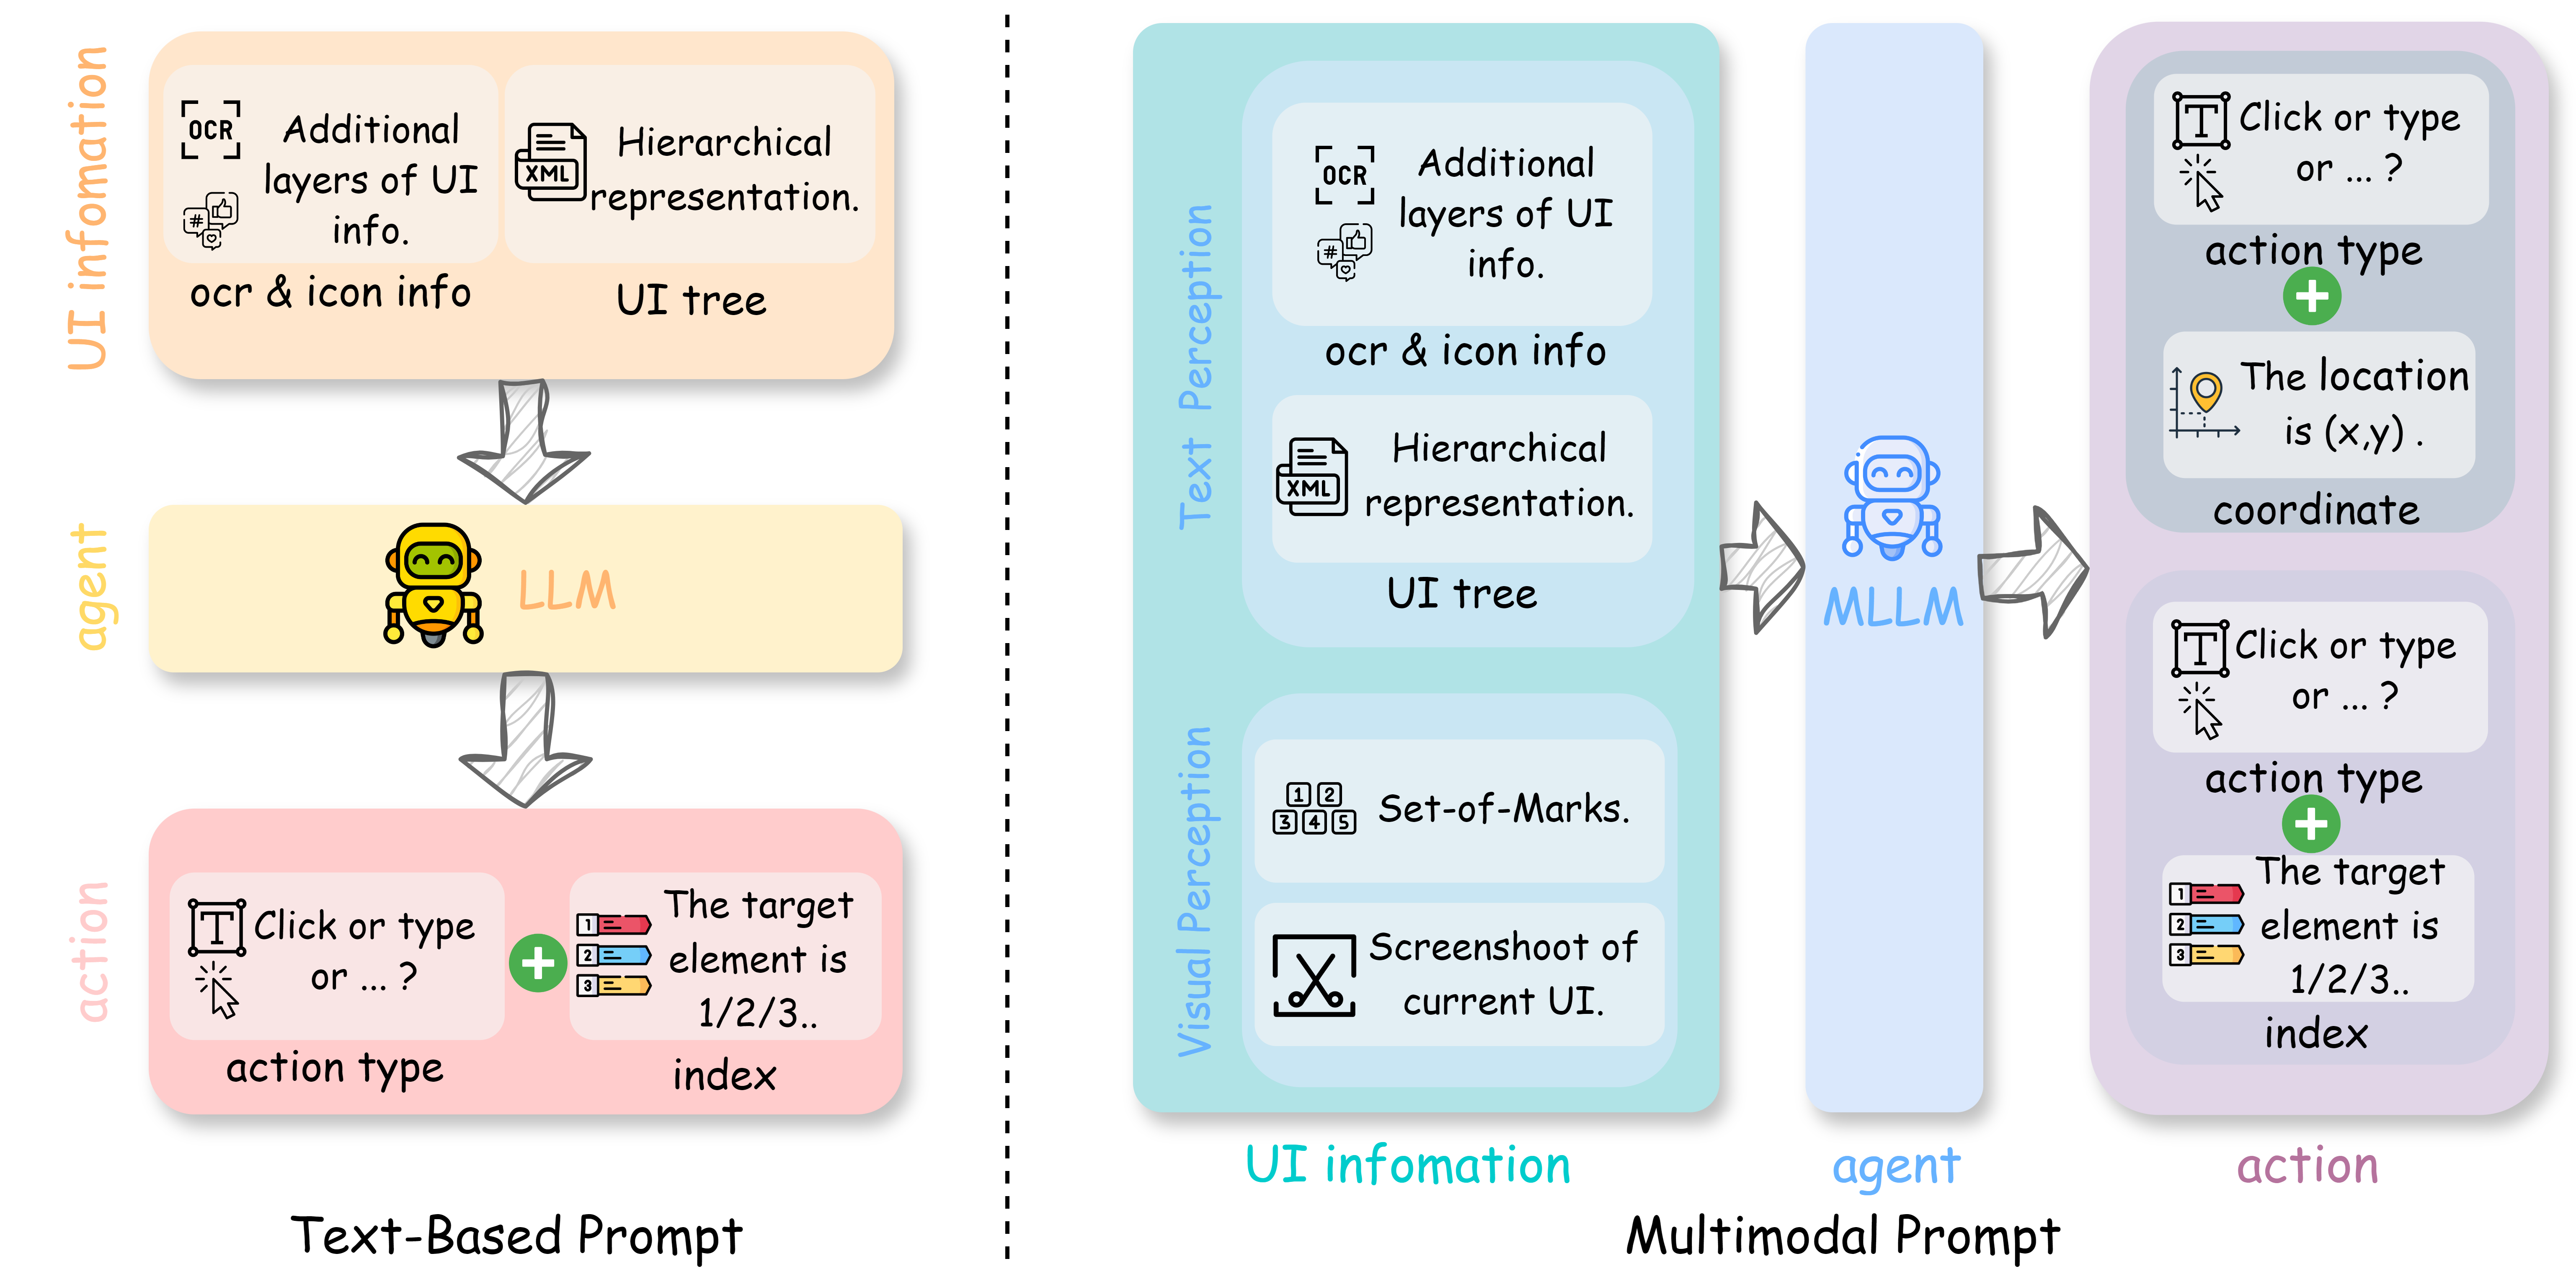
\includegraphics[width=0.95\linewidth]{figures/pe_llm_vs_mllm.drawio.png}
    \caption{Comparison between text-based prompt and multimodal prompt. In Text-Based Prompt, the LLM processes textual UI information, such as UI tree structures and OCR data, to determine the action type (index). In contrast, Multimodal Prompt integrates screenshot data with supplementary UI information to facilitate decision-making by the agent. The MLLM can then pinpoint the action location using either coordinates or indices.}
    \label{fig:pe_llm_vs_mllm}
\end{figure*}


LLMs like the GPT series~\cite{radford2018gpt1,radford2019gpt2,brown2020gpt3} have demonstrated remarkable capabilities in understanding and generating human-like text. These models have revolutionized natural language processing by leveraging massive amounts of data to learn complex language patterns and representations.

Prompt engineering is the practice of designing input prompts to effectively guide LLMs to produce desired outputs for specific tasks~\cite{wei2022chain, yao2024tree, chen2022program}. By carefully crafting the prompts, users can influence the model's behavior without the need for additional training or fine-tuning. This approach allows for leveraging the general capabilities of pre-trained models to perform a wide range of tasks by simply providing appropriate instructions or examples in the prompt.

In the context of phone automation, prompt engineering enables the utilization of general-purpose LLMs to perform automation tasks on mobile devices. Recently, a plethora of works have emerged that apply prompt engineering to achieve phone automation~\cite{wen2023droidbot,yan2023gpt,zhang2023appagent,wang2024mobileagentv1,wang2024mobileagentv2,zhang2024mobileexperts,lu2024omniparser,song2023navigating,taeb2024axnav,yang2024security,liu2024vision, huang2024promptrpa}. These works leverage the strengths of LLMs in natural language understanding and reasoning to interpret user instructions and generate corresponding actions on mobile devices.

The fundamental approach to achieving phone automation through prompt engineering entails the creation of prompts that encapsulate a comprehensive set of information. These prompts should include a detailed task description, such as searching for the best Korean restaurant on Yelp. They also integrate the current UI information of the phone, which may encompass screenshots, SoM, UI tree structures, icon details, and OCR data. Additionally, the prompts should account for the phone's real-time state, including its location, battery level, and keyboard status, as well as any pertinent action history and the range of possible actions (action space). The COT prompt~\cite{wei2022chain,zhang2023igniting} is also a crucial component, guiding the thought process for the next operation. The LLM then analyzes this rich prompt and determines the subsequent action to execute. This methodical process is vividly depicted in Figure~\ref{fig:pe_process}.

This section explores the application of prompt engineering in phone automation, categorizing related works based on the type of prompts used: \textbf{Text-Based Prompt} and \textbf{Multimodal Prompt}. As illustrated in Figure~\ref{fig:pe_llm_vs_mllm}, the approach to automation significantly diverges between these two prompt types. Table~\ref{tab:pe_methods} summarizes notable methods, highlighting their main UI information, the type of model used, and other relevant details such as task types and grounding strategies.

\begin{table*}[htp]
    \centering
    \renewcommand\arraystretch{1.2} % 增加行高以提高可读性
    \caption{Summary of prompt engineering methods for phone GUI agents}
    \resizebox{\textwidth}{!}{ % 调整表格宽度以适应页面宽度
    \begin{tabular}{l c c c c c c c c}
    \toprule
    \textbf{Method} & \textbf{Date} & \textbf{Task Type} & \textbf{Model} & \textbf{Screenshot} & \textbf{SoM} & \textbf{UI tree} & \textbf{\makecell[c]{Icon \\ \& OCR}} & \textbf{Grounding} \\
    % \midrule
    % \makecell[c]{\textbf{\href{https://github.com/MobileLLM/AutoDroid}{DroidBot-}}\\ \textbf{\href{https://github.com/MobileLLM/AutoDroid}{GPT}}\,\cite{wen2023droidbot}\,\githubicon{https://github.com/MobileLLM/AutoDroid}} & 2023.04 & General & ChatGPT & \redcross & \redcross & \greencheck & \redcross & Index \\
    \midrule
    \textbf{\href{https://github.com/MobileLLM/AutoDroid}{DroidBot-GPT}}~\cite{wen2023droidbot} \githubicon{https://github.com/MobileLLM/AutoDroid} & 2023.04 & General & ChatGPT & \redcross & \redcross & \greencheck & \redcross & Index \\
    \midrule
    \textbf{\makecell[l]{Enabling conversa- \\ tional~\cite{wang2023enabling}}} & 2023.04 & \makecell[c]{Screen Under- \\ standing, QA} & PaLM & \redcross & \redcross & \greencheck & \redcross & Index \\
    \midrule
    \textbf{\href{https://github.com/MobileLLM/AutoDroid}{AutoDroid}}~\cite{wen2024autodroid} \githubicon{https://github.com/MobileLLM/AutoDroid} & 2023.09 & General & GPT-4, GPT-3.5 & \redcross & \redcross & \greencheck & \redcross & Index \\
    \midrule
    \textbf{\href{https://github.com/zzxslp/MM-Navigator}{MM-Navigator}}~\cite{yan2023gpt} \githubicon{https://github.com/zzxslp/MM-Navigator} & 2023.11 & General & GPT-4V & \greencheck & \redcross & \redcross & \greencheck & Index \\
    \midrule
    \textbf{\href{https://github.com/AkimotoAyako/VisionTasker}{VisionTasker}}~\cite{song2024visiontasker} \githubicon{https://github.com/AkimotoAyako/VisionTasker} & 2023.12 & Manual Teaching & GPT-4 & \redcross & \greencheck & \greencheck & \greencheck & Index \\
    \midrule
    \textbf{\href{https://github.com/TencentQQGYLab/AppAgent}{AppAgent}}~\cite{zhang2023appagent} \githubicon{https://github.com/TencentQQGYLab/AppAgent} & 2023.12 & General & GPT-4 & \greencheck & \greencheck & \greencheck & \greencheck & Index \\
    \midrule
    \textbf{\href{https://github.com/mobilegptsys/MobileGPT}{MobileGPT}}~\cite{lee2023exploremobilegpt} \githubicon{https://github.com/mobilegptsys/MobileGPT} & 2023.12 & General & GPT-3.5, GPT-4 & \redcross & \redcross & \greencheck & \redcross & Index \\
    \midrule
    \textbf{\href{https://github.com/X-PLUG/MobileAgent}{Mobile-Agent}}~\cite{wang2024mobileagentv1} \githubicon{https://github.com/X-PLUG/MobileAgent} & 2024.01 & General & GPT-4V & \greencheck & \redcross & \redcross & \greencheck & Coordinate \\
    \midrule
    \textbf{AXNav}~\cite{taeb2024axnav} & 2024.05 & Bug Testing & GPT-4 & \redcross & \redcross & \greencheck & \greencheck & Index \\
    \midrule
    \textbf{\href{https://github.com/X-PLUG/MobileAgent}{Mobile-Agent-v2}}~\cite{wang2024mobileagentv2} \githubicon{https://github.com/X-PLUG/MobileAgent} & 2024.06 & General & GPT-4V & \greencheck & \redcross & \redcross & \greencheck & Coordinate \\
    \midrule
    \textbf{\href{https://showlab.github.io/GUI-Narrator/}{GUI Narrator}}~\cite{wu2024gui} \githubicon{https://showlab.github.io/GUI-Narrator/} & 2024.06 & \makecell[c]{GUI Video \\ Captioning} & \makecell[c]{GPT-4o, \\ QwenVL-7B} & \greencheck & \greencheck & \redcross & \redcross & Index \\
    \midrule
    \textbf{MobileExpert}~\cite{zhang2024mobileexperts} & 2024.07 & General & GPT-4V & \greencheck & \redcross & \redcross & \redcross & Coordinate \\
    \midrule
    \textbf{\href{https://github.com/testtestA6/VisionDroid}{VisionDroid}}~\cite{liu2024vision} \githubicon{https://github.com/testtestA6/VisionDroid} & 2024.07 & \makecell[c]{Non-Crash Func-\\tional Bug Detection} & GPT-4 & \greencheck & \greencheck & \greencheck & \redcross & Index \\
    \midrule
    \textbf{AppAgent v2}~\cite{li2024appagentv2} & 2024.08 & General & GPT-4 & \greencheck & \greencheck & \greencheck & \greencheck & \makecell[c]{Coordinate,\\ Index} \\
    \midrule
    \textbf{OmniParser}~\cite{lu2024omniparser} & 2024.08 & General & GPT-4V & \greencheck & \greencheck & \redcross & \greencheck & Index \\
    \midrule
    \textbf{\href{https://x-plug.github.io/MobileAgent/}{Mobile-Agent-E}}~\cite{wang2025mobile} \githubicon{https://x-plug.github.io/MobileAgent/} & 2025.01 & General & \makecell[c]{GPT-4o, Claude \\-3.5,  Gemini-1.5} & \greencheck & \redcross & \redcross & \greencheck & Coordinate \\
    \midrule
    \textbf{\href{https://x-plug.github.io/MobileAgent/}{Mobile-Agent-V}}~\cite{wang2025mobileagentv} \githubicon{https://x-plug.github.io/MobileAgent/} & 2025.02 & General & \makecell[c]{GPT-4o} & \greencheck & \redcross & \redcross & \greencheck & Coordinate \\
    \midrule
    \textbf{\href{https://lgy0404.github.io/LearnAct}{LearnAct}}~\cite{liu2025learnact} \githubicon{https://lgy0404.github.io/LearnAct} & 2025.02 & General & \makecell[c]{Gimini-1.5} & \greencheck & \redcross & \redcross & \redcross & Coordinate \\
    \bottomrule
    \end{tabular}
    } % 结束 resizebox
    \label{tab:pe_methods}
\end{table*}

\subsubsection{Text-Based Prompting}
\label{subsubsec: Text-Based Prompt}

In the domain of text-based prompt automation, the primary architecture involves a single text-modal LLM serving as the agent for mobile device automation. This agent operates by interpreting UI information presented in the form of a UI tree. It is important to note that, to date, the approaches discussed have primarily utilized UI tree data and have not extensively incorporated OCR text and icon information. We believe that solely relying on OCR and icon information is insufficient for fully representing screen UI information; instead, as demonstrated in Mobile-agent-v2~\cite{wang2024mobileagentv2}, they are best used as auxiliary information alongside screenshots. These text-based prompt agents make decisions by selecting elements from a list of candidates based on the textual description of the UI elements. For instance, to initiate a search, the LLM would identify and select the search button by its index within the UI tree rather than its screen coordinates, as depicted in Figure~\ref{fig:pe_llm_vs_mllm}.

The study by Enabling Conversational~\cite{wang2023enabling} marked a significant step in this field. It explored the use of task descriptions, action spaces, and UI trees to map instructions to UI actions. However, it focused solely on the execution of individual instructions without delving into sequential decision-making processes.
DroidBot-GPT~\cite{wen2023droidbot} is a landmark in applying pre-trained language models to app automation. It is the first to explore the use of LLMs for app automation without requiring modifications to the app or the model. DroidBot-GPT perceives UI trees, which are structural representations of the app's UI, and integrates user-provided tasks along with action spaces and output requirements. This allows the model to engage in sequential decision-making and automate tasks effectively. 
AutoDroid~\cite{wen2024autodroid} takes this concept further. It employs a UI Transition Graph (UTG) generated through random exploration to create an App Memory. This memory, combined with the commonsense knowledge of LLMs, enhances decision-making and significantly advances the capabilities of phone GUI agents.
MobileGPT~\cite{lee2023exploremobilegpt} introduces a hierarchical decision-making process. It simulates human cognitive processes—exploration, selection, derivation, and recall—to augment the efficiency and reliability of LLMs in mobile task automation.
Lastly, AXNav~\cite{taeb2024axnav} showcases an innovative application of Prompt Engineering in accessibility testing. AXNav interprets natural language instructions and executes them through an LLM, streamlining the testing process and improving the detection of accessibility issues, thus aiding the manual testing workflows of QA professionals.

Each of these contributions, while unique in their approach, is united by the common thread of Prompt Engineering. They demonstrate the versatility and potential of text-based prompt automation in enhancing the interaction between LLMs and mobile applications.

\subsubsection{Multimodal Prompting}
\label{subsubsec: Multimodal Prompt}

With the advancement of large pre-trained models, Multimodal Large Language Models (MLLMs) have demonstrated exceptional performance across various domains~\cite{achiam2023gpt,li2023blip,ye2023mplug,wang2023cogvlm,Qwen-VL,liu2024visual,Qwen2VL,chen2024internvl,chen2024far,koh2024visualwebarena,zheng2023synapse}, significantly contributing to the evolution of phone automation. Unlike text-only models, multimodal models integrate visual and textual information, addressing limitations such as the inability to access UI trees, missing control information, and inadequate global screen representation. By leveraging screenshots for decision-making, multimodal models facilitate a more natural simulation of human interactions with mobile devices, enhancing both accuracy and robustness in automated operations.

The fundamental framework for multimodal phone automation is illustrated in Figure~\ref{fig:pe_llm_vs_mllm}. Multimodal prompts integrate visual perception (\textit{e.g., screenshots}) and textual information (\textit{e.g., UI tree, OCR, and icon data}) to guide MLLMs in generating actions. The action outputs can be categorized into two methods: \textbf{SoM-Based Indexing Methods} and \textbf{Direct Coordinate Output Methods}. These methods define how the agent identifies and interacts with UI elements, either by referencing annotated indices or by pinpointing precise coordinates.


\noindent\textbf{SoM-Based Indexing Methods.}
SoM-based methods involve annotating UI elements with unique identifiers within the screenshot, allowing the MLLM to reference these elements by their indices when generating actions. This approach mitigates the challenges associated with direct coordinate outputs, such as precision and adaptability to dynamic interfaces.
MM-Navigator~\cite{yan2023gpt} represents a breakthrough in zero-shot GUI navigation using GPT-4V~\cite{achiam2023gpt}. By employing SoM prompting~\cite{yang2023setofmark}, MM-Navigator annotates screenshots through OCR and icon recognition, assigning unique numeric IDs to actionable widgets. This enables GPT-4V to generate indexed action descriptions rather than precise coordinates, enhancing action execution accuracy.
Building upon the SoM-based approach, AppAgent~\cite{zhang2023appagent} integrates autonomous exploration and human demonstration observation to construct a comprehensive knowledge base. This framework allows the agent to navigate and operate smartphone applications through simplified action spaces, such as tapping and swiping, without requiring backend system access. Tested across 10 different applications and 50 tasks, AppAgent showcases superior adaptability and efficiency in handling diverse high-level tasks, further advancing multimodal phone automation.
OmniParser~\cite{lu2024omniparser} enhances the SoM-based method by introducing a robust screen parsing technique. It combines fine-tuned interactive icon detection models and functional captioning models to convert UI screenshots into structured elements with bounding boxes and labels. This comprehensive parsing significantly improves GPT-4V's ability to generate accurately grounded actions, ensuring reliable operation across multiple platforms and applications.
GUI Narrator~\cite{wu2024gui} utilizes video captioning to guide the VLM, aiding in the deeper understanding of GUI operations. The framework uses the mouse cursor as a visual prompt, highlighting it with a green bounding box to enhance the VLM's interpretative abilities with high-resolution screenshots. By extracting screenshots from before and after GUI actions occur in the video as keyframes, it provides temporal and spatial logic to the action screenshots. These are combined into prompts to further guide the VLM in producing accurate action descriptions, thereby improving its performance.



\noindent\textbf{Direct Coordinate Output Methods.}
Direct coordinate output methods enable MLLMs to determine the exact (x, y) positions of UI elements from screenshots, facilitating precise interactions without relying on indexed references. This approach leverages the advanced visual grounding capabilities of MLLMs to interpret and interact with the UI elements directly.
VisionTasker~\cite{song2024visiontasker} introduces a two-stage framework that combines vision-based UI understanding with LLM task planning. Utilizing models like YOLOv8~\cite{varghese2024yolov8} and PaddleOCR~\cite{du2020pp}, VisionTasker parses screenshots to identify widgets and textual information, transforming them into natural language descriptions. This structured semantic representation allows the LLM to perform step-by-step task planning, enhancing the accuracy and practicality of automated mobile task execution.
The Mobile-Agent series~\cite{wang2024mobileagentv1, wang2024mobileagentv2} leverages visual perception tools to accurately identify and locate both visual and textual UI elements within app screenshots. Mobile-Agent-v1 utilizes coordinate-based actions, enabling precise interaction with UI elements. Mobile-Agent-v2 extends this by introducing a multi-agent architecture comprising planning, decision, and reflection agents.
Mobile-Agent-E~\cite{wang2025mobile} optimizes the multi-agent architecture by detailing the responsibilities of each agent. It also introduces a long-term memory mechanism through the design of a Self-Evolution Module, which accumulates experience and enables agents to evolve, thereby enhancing adaptability to new tasks.
MobileExperts~\cite{zhang2024mobileexperts} advances the direct coordinate output method by incorporating tool formulation and multi-agent collaboration. This dynamic, tool-enabled agent team employs a dual-layer planning mechanism to efficiently execute multi-step operations while reducing reasoning costs by approximately 22\%. By dynamically assembling specialized agents and utilizing reusable code block tools, MobileExperts demonstrates enhanced intelligence and operational efficiency in complex phone automation tasks.
Unlike AppAgent, AppAgent v2~\cite{li2024appagentv2} integrates parsers with visual features and employs UI element coordinates along with Index information, creating a more flexible action space. This allows the agent to manage dynamic interfaces and non-standard UI elements more adeptly, thereby enhancing its adaptability to various complex tasks.
VisionDroid~\cite{liu2024vision} applies MLLMs to automated GUI testing, focusing on detecting non-crash functional bugs through vision-based UI understanding. By aligning textual and visual information, VisionDroid enables the MLLM to comprehend GUI semantics and operational logic, employing step-by-step task planning to enhance bug detection accuracy. Evaluations across multiple datasets and real-world applications highlight VisionDroid's superior performance in identifying and addressing functional bugs.


While multimodal prompt strategies have significantly advanced phone automation by integrating visual and textual data, they still face notable challenges. Approaches that do not utilize SoM maps and instead directly output coordinates rely heavily on the MLLM's ability to accurately ground UI elements for precise manipulation. Although recent innovations~\cite{wang2024mobileagentv2,zhang2024mobileexperts,liu2024vision} have made progress in addressing the limitations of MLLMs' grounding capabilities, there remains considerable room for improvement. Enhancing the robustness and accuracy of UI grounding is essential to achieve more reliable and scalable phone automation.


\subsection{Training-Based Models}
\label{subsec:training_based}

The subsequent sections delve into these approaches, discussing the development of task-specific model architectures, supervised fine-tuning strategies and reinforcement learning techniques in both general-purpose and Phone UI-specific scenarios.

\begin{table*}[htp]
    \centering
    \renewcommand\arraystretch{1.2} % 增加行高以提高可读性
    \caption{Summary of task-specific model architectures}
    \resizebox{\textwidth}{!}{ % 调整表格宽度以适应页面宽度
    \begin{tabular}{l c c c c c}
    \toprule
    \textbf{Method} & \textbf{Date} & \textbf{Task Type} & \textbf{Backbone} & \textbf{Size} & \textbf{Contributions} \\
    \midrule
    \textbf{\href{https://github.com/cooelf/Auto-GUI}{Auto-GUI}}~\cite{zhang2023youautoui} \githubicon{https://github.com/cooelf/Auto-GUI} & 2023.09 & General & N/A & \makecell[c]{60M / \\ 200M / \\ 700M} & \makecell[c]{Direct screen interaction; \\ Chain-of-action; Action \\ histories and future plans} \\
    \midrule
    \textbf{\href{https://github.com/THUDM/CogVLM}{CogAgent}}~\cite{hong2024cogagent} \githubicon{https://github.com/THUDM/CogVLM} & 2023.12 & General & CogVLM & 18B & \makecell[c]{High-res input ($1120 \times 1120$); \\ Specialized in GUI understanding} \\
    \midrule
    \textbf{\href{https://github.com/WebVLN/WebVLN}{WebVLN-Net}}~\cite{chen2024webvln} \githubicon{https://github.com/WebVLN/WebVLN} & 2023.12 & \makecell[c]{Screen Under- \\ standing, QA} & N/A & N/A & \makecell[c]{Web navigation with \\ visual and HTML content} \\
    \midrule
    \textbf{\href{https://github.com/google-research-datasets/screen_qa}{ScreenAI}}~\cite{baechler2024screenai} \githubicon{https://github.com/google-research-datasets/screen_qa} & 2024.02 & \makecell[c]{Screen Under- \\ standing, QA} & N/A & 4.6B & \makecell[c]{UI and infographic under-\\standing; Flexible patching} \\
    \midrule
    \makecell[l]{\textbf{\href{https://github.com/xbmxb/CoCo-Agent}{CoCo-Agent}}~\cite{ma2024coco}\,\githubicon{https://github.com/xbmxb/CoCo-Agent}} & 2024.02 & General & \makecell[c]{LLaVA \\(LLaMA-2-\\chat-7B, CLIP)} & N/A & \makecell[c]{Comprehensive perception;\\ Conditional action prediction; \\Enhanced automation} \\
    \midrule
    \textbf{\href{https://github.com/apple/ml-ferret/tree/main/ferretui}{Ferret-UI}}~\cite{you2024ferret} \githubicon{https://github.com/apple/ml-ferret/tree/main/ferretui} & 2024.04 & \makecell[c]{Screen Under- \\ standing, Referring} & Ferret & N/A & \makecell[c]{"Any resolution" tech-niques; \\Precise referring and grounding} \\
    \midrule
    \textbf{LVG}~\cite{qian2024visualgrounding} & 2024.06 & \makecell[c]{Screen Under- \\ standing, Grounding} & \makecell[c]{SWIN Trans-\\former, BERT} & N/A & \makecell[c]{Visual UI grounding; Layout-\\guided contrastive learning} \\
    \midrule
    \makecell[l]{\textbf{\href{https://github.com/aburns4/textualforesight}{Textual}}\\ \textbf{\href{https://github.com/aburns4/textualforesight}{Foresight}}\,\cite{burns2024tell}\,\githubicon{https://github.com/aburns4/textualforesight}} & 2024.06 & \makecell[c]{Screen Under- \\ standing, Referring} & BLIP-2 & N/A & \makecell[c]{Predict UI state;\\ UI representation learning} \\
    \midrule
    \textbf{MobileFlow}~\cite{nong2024mobileflow} & 2024.07 & General & Qwen-VL-Chat & 21B & \makecell[c]{Hybrid visual encoders; Variable \\resolutions; Multilingual support} \\
    \midrule
    \textbf{UI-Hawk}~\cite{zhang2024ui-hawk} & 2024.08 & \makecell[c]{Screen Under- \\ standing, Grounding} & N/A & N/A & \makecell[c]{History-aware encoder;\\ Screen stream processing; \\FunUI benchmark} \\
    \midrule
    \textbf{Ferret-UI 2}~\cite{li2024ferretui2masteringuniversal} & 2024.10 & \makecell[c]{Screen Under- \\ standing, Referring} & Ferret & N/A & \makecell[c]{Multi-platform; \\High-resolution encoding} \\
    \midrule
    \textbf{\href{https://github.com/OS-Copilot/OS-Atlas}{OS-Atlas}}~\cite{wu2024atlas} \githubicon{https://github.com/OS-Copilot/OS-Atlas} & 2024.10 & \makecell[c]{Screen Under- \\ standing, Grounding} & \makecell[c]{Qwen2-VL,\\ InternVL-2} & \makecell[c]{4B / 7B} & \makecell[c]{Grounding data synthesis;\\ Largest GUI grounding corpus} \\
    \midrule
    \textbf{\href{https://github.com/showlab/ShowUI}{ShowUI}}~\cite{lin2024showui} \githubicon{https://github.com/showlab/ShowUI} & 2024.11 & General & Qwen2-VL & 2B & \makecell[c]{Visual tokens selection; \\Cross-modal understanding} \\
    \midrule
    \textbf{\href{https://github.com/xlang-ai/aguvis}{Aguvis}}~\cite{xu2024aguvis} \githubicon{https://github.com/xlang-ai/aguvis} & 2024.12 & General & Qwen2-VL & \makecell[c]{7B / \\ 72B} & \makecell[c]{Comprehensive data pipeline; \\Two-stage training;Cross-platform} \\
    \midrule
    \textbf{\href{https://github.com/AriaUI/Aria-UI}{Aria-UI}}~\cite{yang2024aria} \githubicon{https://github.com/AriaUI/Aria-UI} & 2024.12 & \makecell[c]{Screen Under- \\ standing, Grounding} & Aria & 3.9B & \makecell[c]{Diversified dataset pipeline;\\ Multimodal dynamic action history} \\
    \midrule
    \textbf{\href{https://github.com/bytedance/UI-TARS}{UI-TARS}}~\cite{qin2025ui} \githubicon{https://github.com/bytedance/UI-TARS} & 2025.01 & General & Qwen2-VL & \makecell[c]{2B / 7B / \\ 72B} & \makecell[c]{System-2 Reasoning; Online boot-\\strapping; Reflection tuning} \\
    \midrule
    \textbf{\href{https://gui-bee.github.io/}{GUI-Bee}}~\cite{fan2025gui} \githubicon{https://gui-bee.github.io/} & 2025.01 & \makecell[c]{Screen Under- \\ standing, Grounding} & \makecell[c]{SeeClick, \\ UIX-7B, \\ Qwen-GUI} & N/A & \makecell[c]{Model-Environment alignment;\\ Self-exploratory Data} \\
    \bottomrule
    % 多平台支持;高分辨率图像编码;高质量多模态数据生成方法
    \end{tabular}
    } % 结束 resizebox
    \label{tab:gui_llm_architectures}
\end{table*}

\subsubsection{Task-Specific LLM-based Agents}
\label{subsubsec:task_specific_model_architectures}

To advance AI agents for phone automation, significant efforts have been made to develop Task Specific Model Architectures that are tailored to understand and interact with GUIs by integrating visual perception with language understanding. These models address unique challenges posed by GUI environment, such as varying screen sizes, complex layouts, and diverse interaction patterns. A summary of notable Task Specific Model Architectures is presented in Figure~\ref{tab:gui_llm_architectures}, highlighting their main contributions, domains, and other relevant details.


\noindent\textbf{General-Purpose Models.}
The general-purpose GUI-specific LLMs are designed to handle a wide range of tasks across different applications and interfaces. They focus on enhancing direct GUI interaction, high-resolution visual recognition, and comprehensive perception to improve the capabilities of AI agents in understanding and navigating complex mobile GUIs.
One significant challenge in this domain is enabling agents to interact directly with GUIs without relying on environment parsing or application-specific APIs, which can introduce inefficiencies and error propagation. To tackle this, Auto-GUI~\cite{zhang2023youautoui} presents a multimodal agent that directly engages with the interface. It introduces a chain-of-action technique that leverages previous action histories and future action plans, enhancing the agent's decision-making process and leading to improved performance in GUI control tasks.
High-resolution input is essential for recognizing tiny UI elements and text prevalent in GUIs. CogAgent~\cite{hong2024cogagent} addresses this by employing both low-resolution and high-resolution image encoders within its architecture. Supporting input resolutions up to $1120 \times 1120$, CogAgent effectively recognizes small page elements and text.
Understanding UIs and infographics requires models to interpret complex visual languages and design principles. ScreenAI~\cite{baechler2024screenai} improves upon existing architectures by introducing a flexible patching strategy and a novel textual representation for UIs. During pre-training, this representation teaches the model to interpret UI elements effectively. Leveraging large language models, ScreenAI automatically generates training data at scale, covering a wide spectrum of tasks in UI and infographic understanding.
Enhancing both perception and action response is crucial for comprehensive GUI automation. CoCo-Agent~\cite{ma2024coco} proposes two novel approaches: comprehensive environment perception (CEP) and conditional action prediction (CAP). CEP enhances GUI perception through multiple aspects, including visual channels (screenshots and detailed layouts) and textual channels (historical actions). CAP decomposes action prediction into determining the action type first, then identifying the action target conditioned on the action type.
Addressing the need for effective GUI agents in applications featuring extensive Mandarin content, MobileFlow~\cite{nong2024mobileflow} introduces a multimodal LLM specifically designed for mobile GUI agents. MobileFlow employs a hybrid visual encoder trained on a vast array of GUI pages, enabling it to extract and comprehend information across diverse interfaces. The model incorporates a Mixture of Experts (MoE) and specialized modality alignment training tailored for GUIs.
ShowUI~\cite{lin2024showui} employs the UI-Guided visual tokens selection method, which randomly selects a subset of tokens from each component during training. This approach retains the original positional information while reducing redundant tokens by 33\%, thereby accelerating training speed by 1.4 times. Furthermore, by using interleaved vision-language-action streaming combined with high-quality training data, it significantly improves the training speed and performance of GUI visual agents. Aguvis~\cite{xu2024aguvis} employs a two-stage training method to enhance the generalization and efficiency of GUI agents. It uses single-step task data to train the model's grounding abilities and multi-step task data to develop the model's planning and reasoning capabilities. This approach significantly improves the overall performance of the agents.
UI-TARS~\cite{qin2025ui} employs a more in-depth and structurally robust System-2 reasoning method, combined with online bootstrapping and reflection tuning strategies. This combination effectively assists the model in handling complex tasks in dynamic environments and continuously optimizes overall performance.
Collectively, these general-purpose Task Specific Model Architectures address key challenges in phone automation by enhancing direct GUI interaction, high-resolution visual recognition, comprehensive environment perception, and conditional action prediction. By leveraging multimodal inputs and innovative architectural designs, these models significantly advance the capabilities of AI agents in understanding and navigating complex mobile GUIs, paving the way for more intelligent and autonomous phone automation solutions.


\noindent\textbf{Phone UI-Specific Models.}
Phone UI-Specific Model Architectures have primarily focused on \textit{screen understanding tasks}, which are essential for enabling AI agents to interact effectively with graphical user interfaces. These tasks can be categorized into three main types: \textit{UI grounding}, \textit{UI referring}, and \textit{screen question answering (QA)}. Figure~\ref{fig:ui_understanding_tasks} illustrates the differences between these categories.

\begin{figure*}[ht]
    \centering
    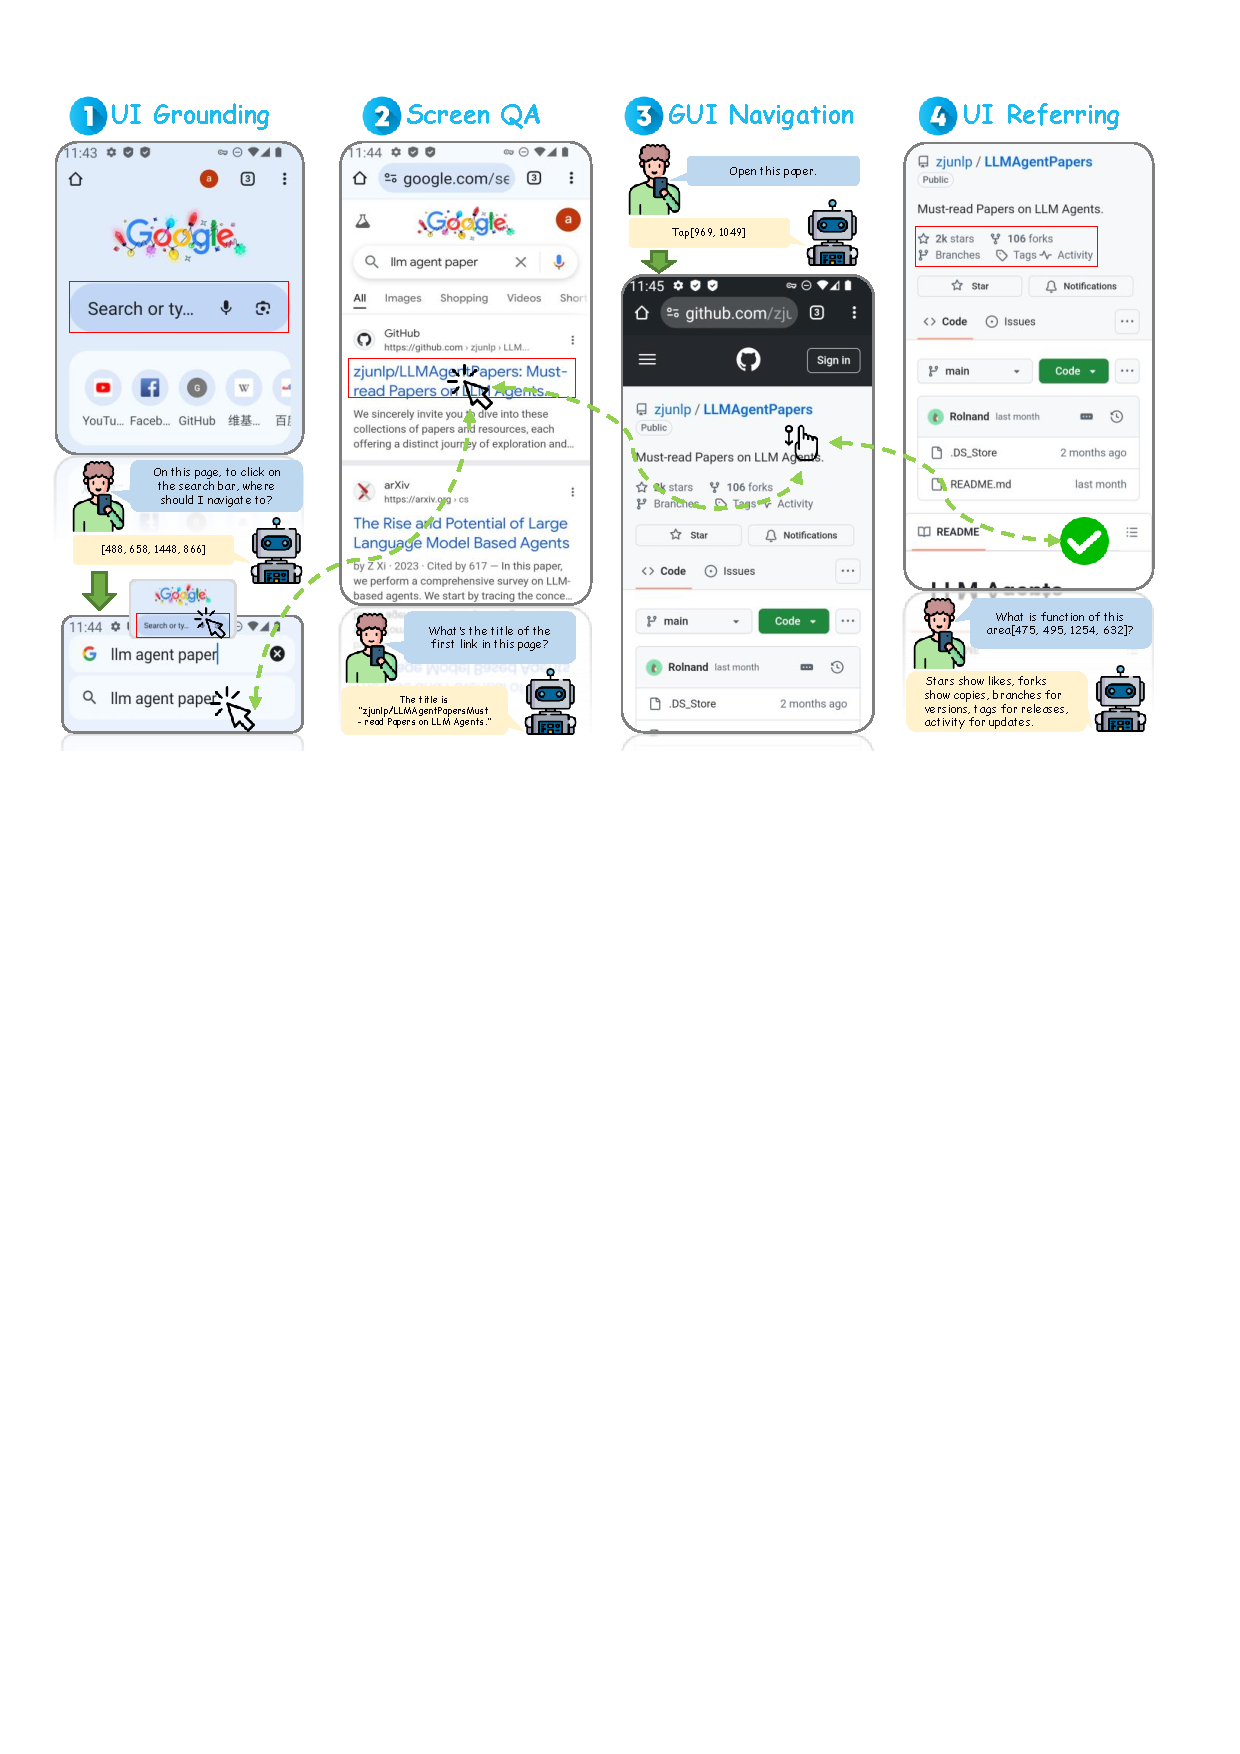
\includegraphics[width=0.95\linewidth]{figures/ui_understanding_tasks.pdf}
    \caption{Illustration of screen understanding tasks. (a) \textit{UI Grounding} involves identifying UI elements corresponding to a given description; (b) \textit{UI Referring} focuses on generating descriptions for specified UI elements; (c) \textit{Screen Question Answering} requires answering questions based on the content of the screen.}
    \label{fig:ui_understanding_tasks}
\end{figure*}

\begin{itemize} 
\item \textbf{UI Grounding}
involves identifying and localizing UI elements on a screen that correspond to a given natural language description. This task is critical for agents to perform precise interactions with GUIs based on user instructions.
MUG~\cite{li2022mug} proposes guiding agent actions through multi-round interactions with users, improving the execution accuracy of UI grounding in complex or ambiguous instruction scenarios. It also leverages user instructions and previous interaction history to predict the next agent action.
LVG (Layout-guided Visual Grounding)~\cite{qian2024visualgrounding} addresses UI grounding by unifying detection and grounding of UI elements within application interfaces. LVG tackles challenges such as \textit{application sensitivity}, where UI elements with similar appearances have different functions across applications, and \textit{context sensitivity}, where the functionality of UI elements depends on their context within the interface. By introducing layout-guided contrastive learning, LVG learns the semantics of UI objects from their visual organization and spatial relationships, improving grounding accuracy.
UI-Hawk~\cite{zhang2024ui-hawk} enhances UI grounding by incorporating a history-aware visual encoder and an efficient resampler to process screen sequences during GUI navigation. By understanding historical screens, UI-Hawk improves the agent's ability to ground UI elements accurately over time. An automated data curation method generates training data for UI grounding, contributing to the creation of the FunUI benchmark for evaluating screen understanding capabilities.
Aria-UI~\cite{yang2024aria} leverages strong MLLMs such as GPT-4o to generate diverse and high-quality element instructions for grounding training. It employs a two-stage training method that incorporates action history in textual or interleaved text-image formats, enabling the model to develop both single-step localization capabilities and multi-step context awareness. This approach demonstrates robust performance and generalization ability across various tasks. Similar research includes GUI-Bee~\cite{fan2025gui}, which autonomously explores environments to collect high-quality data, thereby aligning GUI action grounding models with new environments and significantly enhancing model performance. OS-Atlas~\cite{wu2024atlas} unifies the action space, enabling models to adapt to UI grounding tasks across multiple platforms. Additionally, TAG (Tuning-free Attention-driven Grounding)~\cite{xu2024attention} introduces a method that leverages the inherent attention mechanisms of pre-trained MLLMs to accurately identify and locate elements within a GUI without the need for tuning. Validation shows that this method performs comparably to or even surpasses tuned approaches across multiple benchmark datasets, demonstrating exceptional generalization capabilities. This offers a new perspective for the application of MLLMs in UI grounding.


\item \textbf{UI Referring}
focuses on generating natural language descriptions for specified UI elements on a screen. This task enables agents to explain UI components to users or other agents, facilitating better communication and interaction.
Ferret-UI~\cite{you2024ferret} is a multimodal LLM designed for enhanced understanding of mobile UI screens, emphasizing precise referring and grounding tasks. By incorporating \textit{any resolution} techniques to handle various screen aspect ratios and dividing screens into sub-images for detailed analysis, Ferret-UI generates accurate descriptions of UI elements. Training on a curated dataset of elementary UI tasks, Ferret-UI demonstrates strong performance in UI referring tasks.
Leveraging the Ferret-UI framework, Ferret-UI 2~\cite{li2024ferretui2masteringuniversal} integrates an adaptive N-grid partitioning mechanism. This system enhances image feature extraction by dynamically resizing grids, thereby improving the model's efficiency and accuracy without sacrificing resolution. Additionally, Ferret-UI 2 demonstrates remarkable cross-platform portability. Textual Foresight~\cite{burns2024tell} uses user actions as a bridge, requiring the model to predict the global textual description of the next UI state based on the current UI screen and a local action. With limited training data, the Textual Foresight method achieves superior performance compared to similar models, demonstrating exceptional data efficiency.
UI-Hawk~\cite{zhang2024ui-hawk} also contributes to UI referring by defining tasks that require the agent to generate descriptions for UI elements based on their role and context within the interface. By processing screen sequences and understanding the temporal relationships between screens, UI-Hawk improves the agent's ability to refer to UI elements accurately.

\item \textbf{Screen Question Answering}
involves answering questions about the content and functionality of a screen based on visual and textual information. This task requires agents to comprehend complex screen layouts and extract relevant information to provide accurate answers.
ScreenAI~\cite{baechler2024screenai} specializes in understanding screen UIs and infographics, leveraging the common visual language and design principles shared between them. By introducing a flexible patching strategy and a novel textual representation for UIs, ScreenAI pre-trains models to interpret UI elements effectively. Using large language models to automatically generate training data, ScreenAI covers tasks such as screen annotation and screen QA.
WebVLN~\cite{chen2024webvln} extends vision-and-language navigation to websites, where agents navigate based on question-based instructions and answer questions using information extracted from target web pages. By integrating visual inputs, linguistic instructions, and web-specific content like HTML, WebVLN enables agents to understand both the visual layout and underlying structure of web pages, enhancing screen QA capabilities.
UI-Hawk~\cite{zhang2024ui-hawk} further enhances screen QA by enabling agents to process screen sequences and answer questions based on historical interactions. By incorporating screen question answering as one of its fundamental tasks, UI-Hawk improves the agent's ability to comprehend and reason about screen content over time.
\end{itemize} 


These Phone UI-Specific Model Model Architectures demonstrate the importance of focusing on screen understanding tasks to enhance AI agents' interaction with complex user interfaces. By categorizing these tasks into UI grounding, UI referring, and screen question answering, researchers have developed specialized models that address the unique challenges within each category. Integrating innovative techniques such as layout-guided contrastive learning, history-aware visual encoding, and flexible patching strategies has led to significant advancements in agents' abilities to understand, navigate, and interact with GUIs effectively.

\subsubsection{Supervised Fine-Tuning}
\label{subsubsec:sft}


Supervised fine-tuning has emerged as a crucial technique for enhancing the capabilities of LLMs in GUI tasks within phone automation. By tailoring models to specific tasks through fine-tuning on curated datasets, researchers have significantly improved models' abilities in GUI grounding, optical character recognition (OCR), cross-application navigation, and efficiency. A summary of notable works in this area is presented in Table~\ref{tab:supervised_finetuning}, highlighting their main contributions, domains, and other relevant details.

\begin{table*}[htp]
    \centering
    \renewcommand\arraystretch{1.2} % 增加行高以提高可读性
    \caption{Summary of supervised fine-tuning methods for phone GUI agents}
    \resizebox{\textwidth}{!}{ % 调整表格宽度以适应页面宽度
    \begin{tabular}{l c c c c c}
    \toprule
    \textbf{Method} & \textbf{Date} & \textbf{Task Type} & \textbf{Backbone} & \textbf{Size} & \textbf{Contributions} \\
    \midrule
    \textbf{\href{https://github.com/alipay/mobile-agent}{MobileAgent}}~\cite{ding2024mobileagentsop} \githubicon{https://github.com/alipay/mobile-agent} & 2024.01 & General & Qwen & 7B & \makecell[c]{Standard Operating Procedure; \\Human-machine interaction} \\
    \midrule
    \textbf{\href{https://github.com/njucckevin/SeeClick}{SeeClick}}~\cite{cheng2024seeclick} \githubicon{https://github.com/njucckevin/SeeClick} & 2024.01 & General & Qwen-VL & 9.6B & \makecell[c]{GUI grounding pre-training; \\ScreenSpot benchmark} \\
    \midrule
    \textbf{ReALM}~\cite{moniz2024realm} & 2024.04 & \makecell[c]{Reference \\Resolution} & FLAN-T5 & 80M--3B & \makecell[c]{Formulated reference resolution\\ as language modeling; Improved \\performance on resolving references} \\
    \midrule
    \textbf{\href{https://github.com/yiye3/GUICourse}{GUICourse}}~\cite{chen2024guicourse} \githubicon{https://github.com/yiye3/GUICourse} & 2024.06 & General & \makecell[c]{Qwen-VL,\\ Fuyu-8B, \\MiniCPM-V} & N/A & \makecell[c]{Suite of datasets \\(GUIEnv, GUIAct, GUIChat); \\Enhanced OCR and grounding} \\
    \midrule
    \textbf{\href{https://github.com/OpenGVLab/GUI-Odyssey}{GUI Odyssey}}~\cite{lu2024guiodyssey} \githubicon{https://github.com/OpenGVLab/GUI-Odyssey} & 2024.06 & General & Qwen-VL & N/A & \makecell[c]{Cross-app navigation dataset;\\ Agent with history resampling} \\
    \midrule
    \textbf{IconDesc}~\cite{haque2024infering} & 2024.09 & \makecell[c]{Alt-Text \\Generation} & GPT-3.5 & N/A & \makecell[c]{Generated alt-text for UI \\icons using partial UI data; \\Improved accessibility} \\
    \midrule
    \textbf{\href{https://github.com/SamsungLabs/TinyClick}{TinyClick}}~\cite{pawlowski2024tinyclick} \githubicon{https://github.com/SamsungLabs/TinyClick} & 2024.10 & General & Florence-2 & 0.27B & \makecell[c]{Single-turn agent;\\ Multitask training; \\MLLM-based data augmentation} \\
    \midrule
    \textbf{\href{https://github.com/Reallm-Labs/InfiGUIAgent}{InfiGUIAgent}}~\cite{liu2025infiguiagent} \githubicon{https://github.com/Reallm-Labs/InfiGUIAgent} & 2025.01 & General & Qwen2-VL & 2B & \makecell[c]{Model-Environment alignment;\\ Self-exploratory Data} \\
    \midrule
    \textbf{\href{https://github.com/bytedance/Agent-R}{Agent-R}}~\cite{yuan2025agent} \githubicon{https://github.com/bytedance/Agent-R} & 2025.01 & General & LLama-3.1 & 8B & \makecell[c]{Self-reflection capabilities; \\Real-time error correction} \\
    \bottomrule
    \end{tabular}
    } % 结束 resizebox
    \label{tab:supervised_finetuning}
\end{table*}


% \noindent\textbf{General-Purpose.}
Supervised fine-tuning has been effectively applied to develop more versatile and efficient GUI agents by enhancing their fundamental abilities and GUI knowledge.
One of the fundamental challenges in developing visual GUI agents is enabling accurate interaction with screen elements based solely on visual inputs, known as GUI grounding. SeeClick~\cite{cheng2024seeclick} addresses this challenge by introducing a visual GUI agent that relies exclusively on screenshots for task automation, circumventing the need for extracted structured data like HTML, which can be lengthy and sometimes inaccessible. Recognizing that GUI grounding is a key hurdle, SeeClick enhances the agent's capability by incorporating GUI grounding pre-training. The authors also introduce ScreenSpot, the first realistic GUI grounding benchmark encompassing mobile, desktop, and web environment. Experimental results demonstrate that improving GUI grounding through supervised fine-tuning directly correlates with enhanced performance in downstream GUI tasks.
InfiGUIAgent~\cite{liu2025infiguiagent} is trained using a supervised fine-tuning method and employs the Reference-Augmented Annotation approach to fully leverage spatial information, establishing bidirectional connections between GUI elements and text descriptions, thereby enhancing the model's understanding of GUI visual language. Additionally, the model incorporates Hierarchical Reasoning and Expectation-Reflection Reasoning capabilities, enabling the agent to perform complex reasoning natively, which improves its grounding ability.
Beyond grounding, agents require robust OCR capabilities and comprehensive knowledge of GUI components and interactions to function effectively across diverse applications. GUICourse~\cite{chen2024guicourse} tackles these challenges by presenting a suite of datasets designed to train visual-based GUI agents from general VLMs. The GUIEnv dataset strengthens OCR and grounding abilities by providing 10 million website page-annotation pairs for pre-training and 0.7 million region-text QA pairs for supervised fine-tuning. To enrich the agent's understanding of GUI components and interactions, the GUIAct and GUIChat datasets offer extensive single-step and multi-step action instructions and conversational data with text-rich images and bounding boxes.
As users frequently navigate across multiple applications to complete complex tasks, enabling cross-app GUI navigation becomes essential for practical GUI agents.GUI Odyssey~\cite{lu2024guiodyssey} addresses this need by introducing a comprehensive dataset specifically designed for training and evaluating cross-app navigation agents. The GUI Odyssey dataset comprises 7,735 episodes from six mobile devices, covering six types of cross-app tasks, 201 apps, and 1,399 app combinations. By fine-tuning the Qwen-VL model with a history resampling module on this dataset, they developed OdysseyAgent, a multimodal cross-app navigation agent. Extensive experiments show that OdysseyAgent achieves superior accuracy compared to existing models, significantly improving both in-domain and out-of-domain performance on cross-app navigation tasks.
Efficiency and scalability are also critical considerations, especially for deploying GUI agents on devices with limited computational resources. TinyClick~\cite{pawlowski2024tinyclick} demonstrates that even compact models can achieve strong performance on GUI automation tasks through effective supervised fine-tuning strategies. Utilizing the Vision-Language Model Florence-2-Base, TinyClick focuses on the primary task of identifying the screen coordinates of UI elements corresponding to user commands. By employing multi-task training and Multimodal Large Language Model-based data augmentation, TinyClick significantly improves model performance while maintaining a compact size of 0.27 billion parameters and minimal latency.
MobileAgent~\cite{ding2024mobileagentsop} combines LoRA and SOP methods to effectively reduce computational overhead through low-rank adaptive supervised fine-tuning, while breaking down complex tasks into subtasks to enhance the model's understanding and execution efficiency. At the same time, this approach does not impose additional burdens on inference speed, significantly improving the model's performance and responsiveness.
The performance of agents is often limited by their inability to recover from errors. Agent-R~\cite{yuan2025agent} identifies the first error step in an erroneous trajectory and combines it with a correct trajectory to create a corrected path, thus enabling real-time error correction. By training on self-generated corrected trajectories and using an iterative supervised fine-tuning approach, Agent-R dynamically identifies and rectifies errors, gradually enhancing decision-making abilities. Moreover, under a multi-task training strategy, its training outcomes improve significantly. This method offers new directions for developing more intelligent and adaptable GUI agents.


% \noindent\textbf{Domain-Specific.}
Supervised fine-tuning has also been applied to domain-specific tasks to address specialized challenges in particular contexts, such as reference resolution and accessibility.
In the context of \textbf{Reference Resolution in GUI Contexts}, ReALM~\cite{moniz2024realm} formulates reference resolution as a language modeling problem, enabling the model to handle various types of references, including on-screen entities, conversational entities, and background entities. By converting reference resolution into a multiple-choice task for the LLM, ReALM significantly improves the model's ability to resolve references in GUI contexts.
For \textbf{Accessibility and UI Icons Alt-Text Generation}, IconDesc~\cite{haque2024infering} addresses the challenge of generating informative alt-text for mobile UI icons, which is essential for users relying on screen readers. Traditional deep learning approaches require extensive datasets and struggle with the diversity and imbalance of icon types. IconDesc introduces a novel method using Large Language Models to autonomously generate alt-text with partial UI data, such as class, resource ID, bounds, and contextual information from parent and sibling nodes. By fine-tuning an off-the-shelf LLM on a small dataset of approximately 1.4k icons, IconDesc demonstrates significant improvements in generating relevant alt-text, aiding developers in enhancing UI accessibility during app development.


These works collectively demonstrate that supervised fine-tuning is instrumental in advancing GUI agents for phone automation. By addressing specific challenges through targeted datasets and training strategies—whether enhancing GUI grounding, improving OCR and GUI knowledge, enabling cross-app navigation, or optimizing for accessibility—researchers have significantly enhanced the performance and applicability of GUI agents. The advancements summarized in Figure~\ref{tab:supervised_finetuning} highlight the ongoing efforts and progress in this field, paving the way for more intelligent, versatile, and accessible phone automation solutions capable of handling complex tasks in diverse environment.

\subsubsection{Reinforcement Learning}
\label{subsubsec:rl}


Reinforcement Learning (RL)~\cite{kaelbling1996reinforcement} has emerged as a powerful technique for training agents to interact autonomously with GUIs across various platforms, including phones, web browsers, and desktop environment. Although RL-based approaches for phone GUI agents are relatively few, significant progress has been made in leveraging RL to enhance agent capabilities in dynamic and complex GUI environment. In this section, we discuss RL approaches for GUI agents across different platforms, highlighting their unique challenges, methodologies, and contributions. A summary of notable RL-based methods is presented in Figure~\ref{tab:reinforcement_learning}, which includes specific RL-related features such as the type of RL used (online or offline) and the targeted platform.

\begin{table*}[htp]
    \centering
    \renewcommand\arraystretch{1.2} % 增加行高以提高可读性
    \caption{Summary of reinforcement learning methods for phone GUI agents}
    \resizebox{\textwidth}{!}{ % 调整表格宽度以适应页面宽度
    \begin{tabular}{l c c c c c}
    \toprule
    \textbf{Method} & \textbf{Date} & \textbf{Platform} & \textbf{RL Type} & \textbf{Backbone} & \textbf{Size} \\
    \midrule
    \textbf{\href{https://github.com/DigiRL-agent/digirl}{DigiRL}}~\cite{bai2024digirl} \githubicon{https://github.com/DigiRL-agent/digirl} & 2024.06 & Phone & Online RL & AutoUI-Base & 200M \\
    \midrule
    \textbf{\href{https://github.com/DistRL-lab/distrl-open}{DistRL}}~\cite{wang2024distrl} \githubicon{https://github.com/DistRL-lab/distrl-open} & 2024.10 & Phone & Online RL & T5-based & 1.3B \\
    \midrule
    \textbf{\href{https://xiao9905.github.io/AutoGLM/}{AutoGLM}}~\cite{liu2024autoglm} \githubicon{https://xiao9905.github.io/AutoGLM/} & 2024.11 & \makecell[c]{Phone,\\Web} & Online RL & GLM-4-9B-Base & 9B \\
    \midrule
    \textbf{\href{https://github.com/niuzaisheng/ScreenAgent}{ScreenAgent}}~\cite{niu2024screenagent} \githubicon{https://github.com/niuzaisheng/ScreenAgent} & 2024.02 & PC OS & N/A & CogAgent & 18B \\
    \midrule
    \textbf{\href{https://github.com/Yifan-Song793/ETO}{ETO}}~\cite{song2024trial} \githubicon{https://github.com/Yifan-Song793/ETO} & 2024.03 & Web & \makecell[c]{Offline-to-\\Online RL} & LLaMA-2-7B-Chat & 7B \\
    \midrule
    \textbf{\href{https://github.com/THUDM/AutoWebGLM}{AutoWebGLM}}~\cite{lai2024autowebglm} \githubicon{https://github.com/THUDM/AutoWebGLM} & 2024.04 & Web & \makecell[c]{RL (Curriculum \\Learning, Boot-\\strapped RL)} & ChatGLM3-6B & 6B \\
    \midrule
    \textbf{\href{https://github.com/sentient-engineering/agent-q}{Agent Q}}~\cite{putta2024agentq} \githubicon{https://github.com/sentient-engineering/agent-q} & 2024.08 & Web & Offline RL with MCTS & LLaMA-3-70B & 70B \\
    \midrule
    \textbf{\href{https://github.com/MultifacetedNLP/Web-Agents-Unsupervised}{GLAINTEL}}~\cite{Fereidouni_2024} \githubicon{https://github.com/MultifacetedNLP/Web-Agents-Unsupervised} & 2024.11 & Web & \makecell[c]{RL (Offline-to-\\Online, Hybrid RL)} & Flan-T5 & 0.78B \\
    \midrule
    \textbf{ReachAgent}~\cite{wu2025reachagent} & 2025.02 & Phone & Hybrid RL & MobileVLM~\cite{wu2024mobilevlm} & N/A \\
    \midrule
    \textbf{\href{https://github.com/microsoft/GUI-Agent-RL}{VEM}}~\cite{zheng2025vem} \githubicon{https://github.com/microsoft/GUI-Agent-RL} & 2025.02 & Phone & \makecell[c]{Environment-\\Free RL} & N/A & N/A \\
    \midrule
    \textbf{\href{https://github.com/DigiRL-agent/digiq}{Digi-Q}}~\cite{bai2025digi} \githubicon{https://github.com/DigiRL-agent/digiq} & 2025.02 & Phone & \makecell[c]{Q-Function \\Based RL} & N/A & N/A \\
    \midrule
    \textbf{\href{https://ai-agents-2030.github.io/VSC-RL}{VSC-RL}}~\cite{wu2025vsc} \githubicon{https://ai-agents-2030.github.io/VSC-RL} & 2025.02 & Phone & \makecell[c]{Variational \\Subgoal-\\Conditioned RL} & N/A & N/A \\
    \midrule
    \textbf{\href{https://github.com/lll6gg/UI-R1}{UI-R1}}~\cite{lu2025ui} \githubicon{https://github.com/lll6gg/UI-R1} & 2025.03 & Phone & \makecell[c]{Rule-Based RL} & Qwen2.5-VL & 3B \\
    \bottomrule
    \end{tabular}
    } % 结束 resizebox
    \label{tab:reinforcement_learning}
\end{table*}




\noindent\textbf{Phone Agents.}
Training phone GUI agents using RL presents unique challenges due to the dynamic and complex nature of mobile applications. Agents must adapt to real-world stochasticity and handle the intricacies of interacting with diverse mobile environment. Recent works have addressed these challenges by developing RL frameworks that enable agents to learn from interactions and improve over time.
DigiRL~\cite{bai2024digirl} andDistRL~\cite{wang2024distrl} both tackle the limitations of pre-trained vision-language models (VLMs) in decision-making tasks for device control through GUIs. Recognizing that static demonstrations are insufficient due to the dynamic nature of real-world mobile environment, these works introduce RL approaches to train agents capable of in-the-wild device control.
DigiRL proposes an autonomous RL framework that employs a two-stage training process: an initial offline RL phase to initialize the agent using existing data, followed by an offline-to-online RL phase that fine-tunes the model based on its own interactions. By building a scalable Android learning environment with a VLM-based evaluator, DigiRL identifies key design choices for effective RL in mobile GUI domains. The agent learns to handle real-world stochasticity and dynamism, achieving significant improvements over supervised fine-tuning, with a 49.5\% absolute increase in success rate on the Android-in-the-Wild dataset.
Similarly, DistRL introduces an asynchronous distributed RL framework specifically designed for on-device control agents on mobile devices. To address inefficiencies in online fine-tuning and the challenges posed by dynamic mobile environment, DistRL employs centralized training and decentralized data acquisition. Leveraging an off-policy RL algorithm tailored for distributed and asynchronous data utilization, DistRL improves training efficiency and agent performance by prioritizing significant experiences and encouraging exploration. Experiments show that DistRL achieves a 20\% relative improvement in success rate compared to state-of-the-art methods on general Android tasks.
Building upon these advancements, AutoGLM~\cite{liu2024autoglm} extends the application of RL to both phone and web platforms. AutoGLM presents a series of foundation agents based on the ChatGLM model family, aiming to serve as autonomous agents for GUI control. A key insight from this work is the design of an intermediate interface that separates planning and grounding behaviors, allowing for more agile development and enhanced performance. By employing self-evolving online curriculum RL, AutoGLM enables agents to learn from environmental interactions and adapt to dynamic GUI environment. The approach demonstrates impressive success rates on various benchmarks, showcasing the potential of RL in creating versatile GUI agents across platforms.

Recent advances have brought several innovative approaches to reinforcement learning for phone GUI agents. ReachAgent~\cite{wu2025reachagent} decomposes mobile agent tasks into two sub-tasks: page reaching and page operation, utilizing a two-stage fine-tuning strategy. In the first stage, supervised fine-tuning enables the agent to better perform each sub-task. In the second stage, reinforcement learning is applied to further optimize the agent's overall task completion capabilities, thereby enhancing its performance in complex tasks. VEM~\cite{zheng2025vem} introduces an environment-free RL framework that decouples value estimation from policy optimization using a pretrained Value Environment Model. Unlike traditional RL methods that require costly environment interactions, VEM predicts state-action values directly from offline data, distilling human-like priors about GUI interaction outcomes. This approach avoids compounding errors and enhances resilience to UI changes by focusing on semantic reasoning. Digi-Q~\cite{bai2025digi} presents an approach to train VLM-based action-value Q-functions for device control. Instead of using on-policy RL with actual environment rollouts, Digi-Q trains the Q-function using offline temporal-difference learning on frozen, intermediate-layer features of a VLM. This approach enhances scalability and reduces computational costs compared to fine-tuning the entire VLM. The trained Q-function then uses a Best-of-N policy extraction operator to imitate the best action without requiring environment interaction. VSC-RL~\cite{wu2025vsc} addresses the learning inefficiencies in tackling complex sequential decision-making tasks with sparse rewards and long-horizon dependencies. By reformulating vision-language sequential tasks as a variational goal-conditioned RL problem, VSC-RL optimizes the SubGoal Evidence Lower BOund (SGC-ELBO). This approach maximizes subgoal-conditioned return via RL while minimizing the difference with the reference policy. UI-R1~\cite{lu2025ui} explores how rule-based RL can enhance reasoning capabilities of multimodal large language models for GUI action prediction. Using a small yet high-quality dataset of 136 challenging tasks, UI-R1 introduces a unified rule-based action reward enabling model optimization via Group Relative Policy Optimization (GRPO).

\noindent\textbf{Web Agents.}
Web navigation tasks involve interacting with complex and dynamic web environment, where agents must interpret web content and perform actions to achieve user-specified goals. RL has been employed to train agents that can adapt to these challenges by learning from interactions and improving decision-making capabilities.
ETO~\cite{song2024trial} (Exploration-based Trajectory Optimization) and Agent Q~\cite{putta2024agentq} both focus on enhancing the performance of LLM-based agents in web environment through RL techniques. ETO introduces a learning method that allows agents to learn from their exploration failures by iteratively collecting failure trajectories and using them to create contrastive trajectory pairs for training. By leveraging contrastive learning methods like Direct Preference Optimization (DPO), ETO enables agents to improve performance through an iterative cycle of exploration and training. Experiments on tasks such as WebShop demonstrate that ETO consistently outperforms baselines, highlighting the effectiveness of learning from failures.
Agent Q combines guided Monte Carlo Tree Search (MCTS) with a self-critique mechanism and iterative fine-tuning using an off-policy variant of DPO. This framework allows LLM agents to learn from both successful and unsuccessful trajectories, improving generalization in complex, multi-step reasoning tasks. Evaluations on the WebShop environment and real-world booking scenarios show that Agent Q significantly improves success rates, outperforming behavior cloning and reinforcement learning fine-tuned baselines.
AutoWebGLM~\cite{lai2024autowebglm} contributes to this domain by developing an LLM-based web navigating agent built upon ChatGLM3-6B. To address the complexity of HTML data and the versatility of web actions, AutoWebGLM introduces an HTML simplification algorithm to represent webpages succinctly. The agent is trained using a hybrid human-AI method to build web browsing data for curriculum training and is further enhanced through reinforcement learning and rejection sampling. AutoWebGLM demonstrates performance superiority on general webpage browsing tasks, achieving practical usability in real-world services.
GLAINTEL~\cite{Fereidouni_2024} effectively utilizes human experience and the adaptive capabilities of reinforcement learning by integrating human demonstrations with reinforcement learning methods. This approach achieves superior performance in complex product search tasks.
Collectively, these works demonstrate how RL techniques can be applied to web agents to improve their ability to navigate and interact with complex web environment. By learning from interactions, failures, and leveraging advanced planning methods, these agents exhibit enhanced reasoning and decision-making capabilities.


\noindent\textbf{PC OS Agents.}
In desktop environment, agents face the challenge of interacting with complex software applications and operating systems, requiring precise control actions and understanding of GUI elements. RL approaches in this domain focus on enabling agents to perform multi-step tasks and adapt to the intricacies of desktop GUIs.
ScreenAgent~\cite{niu2024screenagent} constructs an environment where a Vision Language Model (VLM) agent interacts with a real computer screen via the VNC protocol. By observing screenshots and manipulating the GUI through mouse and keyboard actions, the agent operates within an automated control pipeline that includes planning, acting, and reflecting phases. This design allows the agent to continuously interact with the environment and complete multi-step tasks. ScreenAgent introduces the ScreenAgent Dataset, which collects screenshots and action sequences for various daily computer tasks. The trained model demonstrates computer control capabilities comparable to GPT-4V and exhibits precise UI positioning capabilities, highlighting the potential of RL in desktop GUI automation.
AssistGUI~\cite{gao2023assistgui} develops an LLM-based reinforcement learning framework called Actor-Critic Embodied Agent (ACE). This framework automates desktop GUI through visual analysis, reasoning, and action generation, significantly improving task success rates. Additionally, it introduces a novel benchmarking framework to evaluate a model's ability to complete complex tasks on desktop platforms using mouse and keyboard operations. This advancement offers a new direction for future research in desktop GUI automation.



Reinforcement Learning has proven to be a valuable approach for training GUI agents across various platforms, enabling them to learn from interactions with dynamic environment and improve their performance over time. By leveraging RL techniques, these agents can adapt to real-world stochasticity, handle complex decision-making tasks, and exhibit enhanced autonomy in phone, web, and desktop environment. The works discussed in this section showcase the progress made in developing intelligent and versatile GUI agents through RL, paving the way for enhanced automation and user interaction across diverse platforms.